\documentclass{beamer}
%\usepackage{beamerfoils}
\mode<presentation>
{
  \usetheme{Darmstadt}
}
%\usepackage[czech]{babel}
%\usepackage[latin2]{inputenc}
\usepackage{ucs}
\usepackage[utf8x]{inputenc}
\usepackage[czech]{babel}
\usepackage{times}
\usepackage[T1]{fontenc}
\usepackage{xspace}

\title[]{Fast SAT Solver}
\author[]{Kamil Dudka}
\institute[]{Fakulta informačních technologií\\Vysoké učení technické v Brně}
\begin{document}

% Title frame
\begin{frame}
  \frametitle{Fast SAT Solver}
  \begin{center}
    \vbox{FAKULTA INFORMAČNÍCH TECHNOLOGIÍ\\\vspace{.2cm}VYSOKÉ UČENÍ TECHNICKÉ V BRNĚ\\\vspace{1cm}}
    
\includegraphics[width=2cm,keepaspectratio]{cls/fit-zp2}
    \vfill
    \vbox{Autor práce\hfill Kamil Dudka}\vspace{.3cm}\vbox{Vedoucí práce\hfill Ing. Jiří Jaroš}
  \end{center}
\end{frame}

\section{SAT Problem}
\begin{frame}[fragile]
  \frametitle{SAT Problem}
  \begin{itemize}
   \item SATisfiability Problem
   \begin{displaymath}
    \begin{array}{l}
     \neg(\neg x_1 \vee x_2)\vee x_3 \wedge\neg(\neg x_1 \Leftrightarrow x_3)\\
     \neg(x_1 \wedge x_2 \wedge x_3)
    \end{array}
   \end{displaymath}
   \smallskip
   \item Jazyk pro zápis formulí
   \begin{verbatim}
          ~(~x1|x2)|x3&(~x1 XOR x3);
          ~(x1 & x2 & x3);
   \end{verbatim}
   \smallskip
   \item Nezávislá interní reprezentace
  \end{itemize}
\end{frame}

\section{SAT Solver}
\begin{frame}
  \frametitle{SAT Solver}
  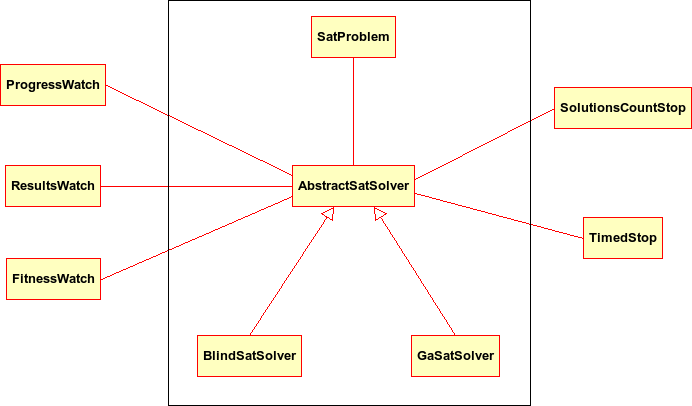
\includegraphics[scale=0.45]{AbstractSatSolver.png}
\end{frame}
\begin{frame}
  \frametitle{SAT Solver - pokračování}
  \begin{itemize}
   \item Automatický restart
   \medskip\item Najde řešení rchleji, pokud zná předem jejich počet
   \medskip\item Lze nastavit maximální čas prohledávání
  \end{itemize}
  \begin{flushright}
    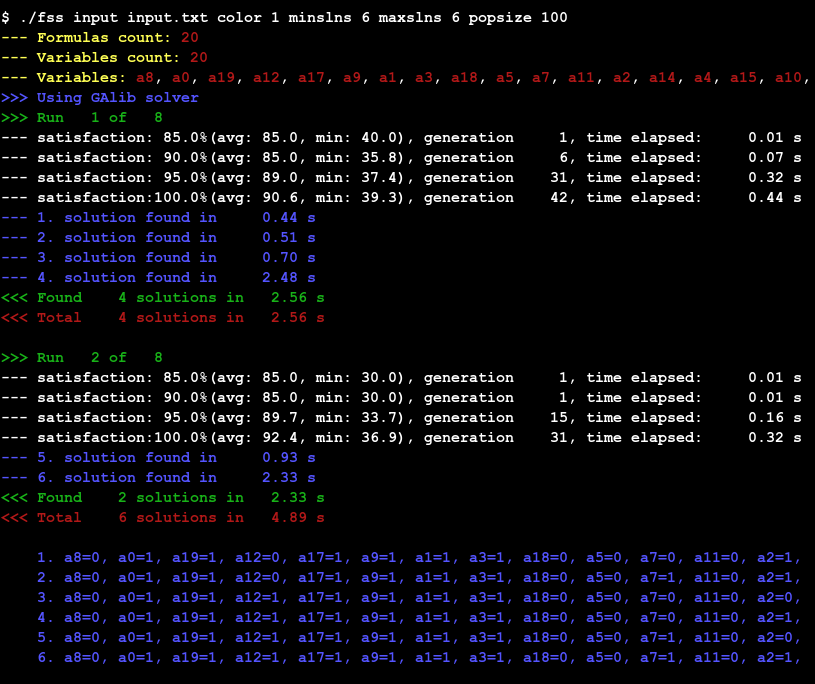
\includegraphics[scale=0.2]{screenshot.png}
  \end{flushright}
\end{frame}

\section{Výsledky}
\begin{frame}
  \frametitle{Výsledky}
  \begin{itemize}
   \item Generátor náhodných SAT problémů
   \item Srovnání GA a slepého prohledávače
   \item Řídící parametry GA
   \bigskip\item Srovnání pro 20 výrokových formulí o 20ti proměnných
    \begin{table}[h]
    \begin{center}
      \begin{tiny}
      \begin{tabular}{|l|r|r|}\hline
        Parametry prohledávání&Počet nalezených řešení&Doba prohledávání\\\hline
        \textit{bez parametru}&3 -- 6&1.29 s\\
        \texttt{ngen 500}&5 -- 6&2.58 s\\
        \texttt{minslns 6}&6&1.29 -- 5.19 s\\
        \texttt{minslns 6 maxslns 6}&6&0.60 -- 5.19 s\\
        \texttt{minslns 6 maxslns 6 time 1000 maxruns 1}&0 -- 6&0.60 -- 1.01 s\\\hline
        \texttt{blind 1}&6&116.07 s\\
        \texttt{blind 1 maxslns 6}&6&92.03 s\\
        \texttt{blind 1 maxtime 60000 stepw 10}&4&60.12 s\\\hline
      \end{tabular} 
      \end{tiny}
    \end{center}
    \label{tabTime}
    \end{table}
  \end{itemize}
%   \begin{itemize}
%    \item Testování knihovny\\
%    {\tiny (testovací programy dodávané spolu s knihovnou)}
%    
%    \bigskip\item Výkon při práci s knihovnou\\
%    {\tiny Při použití sdílené paměti byl výkon testovací aplikace asi \textbf{3-5x nižší} než výkon její nesdílené varianty.}
%    
%    \bigskip\item Omezení knihovny\\
%    {\tiny Ve sdílených objektech nelze používat \textbf{virtuální metody}.}
%   \end{itemize}

\end{frame}

% \section{Budoucnost knihovny}
% \begin{frame}
%   \frametitle{Budoucnost knihovny}
%   \begin{itemize}
%    \item Testování na reálných aplikacích
%    \bigskip\item Alokace a dealokace bloků uvnitř sdíleného segmentu\\
%    {\tiny (garbage collector)}
%    \bigskip\item Synchronizační prostředky pro sdílená data\\
%    {\tiny (implementace monitoru)}
%   \end{itemize}
% 
% \end{frame}

\end{document}

